\chapter{Proof of Concept}
\label{sec:proofofconcept}

% PHP/XEDUB installation: https://ubuntuforums.org/showthread.php?t=525257
%						  https://www.youtube.com/watch?v=OlcsQ8TCU3A
%	> sudo add-apt-repository ppa:ondrej/php
%	> sudo apt-get update
%	> sudo apt-get apache2
% 	> sudo apt-get install php7.1-dev php-pear php7.1-mbstring php7.1-cgi	  			// old... > sudo apt-get install php5-dev php-pear
%	> sudo apt-get install libapache2-mod-php7.0
% 	> sudo pecl install xdebug
% 	> find / -name 'xdebug.so' 2> /dev/null
% 	/usr/lib/php5/20060613/xdebug.so
% 	> sudo gedit /etc/php/7.1/apache2/php.ini		
%		[xdebug]
%		zend_extension=/usr/lib/php/20160303/xdebug.so
%		xdebug.default_enable=1
%		xdebug.idekey=PHPSTORM
%		xdebug.remote_enable=1
%		xdebug.remote_port=9000
%		xdebug.remote_connect_back=1

% Enabling error msg. Set "`display_errors = On"' in:
%	> sudo gedit /etc/php/7.1/apache2/php.ini	

% Change document root:
% 	> sudo gedit /etc/apache2/sites-available/000-default.conf
%	> sudo gedit /etc/apache2/apache2.conf
% 	> sudo /etc/init.d/apache2 restart

% Installing grunt (as npm package):
%	> npm init
%	> npm install grunt --save-dev
%	create Gruntfile and update package.json according to: https://gruntjs.com/getting-started and http://www.wearecube.ch/from-less-to-css-with-grunt-js/
%	> npm install
%	> grunt
%					// > grunt watch &				// grunt watch will be stoped when the commandline closes

% installing composer/twig:
% 	download to project root: https://getcomposer.org
% 	> php composer-setup.php --filename=composer
%	create composer.json in project root. content:
% 		{
%			"require": {
%   			"twig/twig": "1.*",
%			    "twbs/bootstrap": "3.3.7"
%  			}
%		}
%	> php composer.phar install 		or			php composer.phar update
%	> sudo chown www-data:www-data bookinganalyzerimpl/compilation_cache/

% https://nikic.github.io/2011/12/12/How-big-are-PHP-arrays-really-Hint-BIG.html
% installing redis
%	> sudo pecl install redis
%	Adding "extension=redis.so" to php.ini
%	  	> sudo gedit /etc/php/7.1/apache2/php.ini	
%	  	> sudo gedit /etc/php/7.1/cli/php.ini	
% 	> sudo /etc/init.d/apache2 restart
%
%	> wget http://download.redis.io/releases/redis-3.2.8.tar.gz
%	> tar xzf redis-3.2.8.tar.gz
%	> cd redis-3.2.8
%	> make
% 	> ~/programs/redis-3.2.8/src/redis-server
% http://www.codeforge.com/article/214557


% Getting bookinganalyzerimpl to run:
% git clone git@github.com:soultemptation/bookinganalyzerimpl.git
% npm install
% grunt
% php composer.phar install

% Remove duplicates:
%			Find duplicates:
%			> egrep -o '^[^@]+' u611a_10_normalized_geocoded.csv > text.csv 	// Get everything before first @
%			> sort text.csv > text_sorted.csv									// Sort it
%			> uniq -d text_sorted.csv > text2_duplicates.csv					// Remove duplicates
% 	> tac u611a_10_normalized_geocoded.csv | sort -k1,1 -r -u -t@ > text5.csv
%	> tac text5.csv > text6.csv
%	Move last line of text6.csv to the beginning

\section{Datenvorbereitung}
\label{sec:proofofconcept:datenvorbereitung}

% Feature selection
% https://en.wikipedia.org/wiki/Feature_selection
% http://dollar.biz.uiowa.edu/~street/research/dmoc.pdf
% http://www.jmlr.org/papers/volume3/guyon03a/guyon03a.pdf

Die Daten müssen für die Verwendung im Proof of Concept vorbereitet werden. Dazu wurden zwei Programme geschrieben um die Daten anzureichern. Die Datentransormationen wurden anschliessend gemäss \cref{sec:recherche:datenvorbereitung} mit dem Programm RapidMiner durchgeführt.

\subsection{Datenerweiterung}
\label{sec:proofofconcept:datenvorbereitung:datenerweiterung}
Die Programme für die Datenanreicherungen sind jeweils eine Kommandozeilen-Software welche hier vorgestellt werden.

\subsubsection{Land, Region, Ortschaft}
\label{sec:proofofconcept:datenvorbereitung:datenerweiterung:landregionortschaft}
Es wurde ein Programm für die Anreicherung vom Land, der Region sowie der Ortschaft der Objekte erstellt. Es erwartet eine \gls{csv} Datei mit einem @-Zeichen als Feldseparator, sowie das Feld "`NREF"' welches in jeder Zeile vorkommen muss und die ID des Objektes beinhaltet. Der Quellcode ist einsehbar in Github unter \url{https://github.com/soultemptation/bookinganalyzerdestinations}.

Die Software verarbeitet Zeile für Zeile der Datei und fügt am Ende drei Felder mit den Namen "`country"', "`region"' und "`place"' an. Um die Daten zu erhalten wird der Such-Service von Interhome angesprochen, welcher die drei Informationen zurückliefert. Als Parameter des Services wird die `NREF"' des Objektes übergeben. 

Es kann sein dass das Objekt bei Interhome nicht mehr vorhanden ist und der Service nichts zurück liefert. Deshalb gibt es nach der Ausführung des Programmes Buchungen welche keine Informationen für das Land, die Region und die Ortschaft besitzen.

Im Programm wird ein Cache verwendet, welcher für jede "`NREF"' das Land, die Region und die Ortschaft zwischenspeichert. Wenn eine "`NREF"' zum zweiten mal angefragt werden soll, können die Daten aus dem Cache bezogen werden und es muss kein weiterer Service Aufruf durchgeführt werden. Für die 133'001 Buchungen mussten dank des Caches nur 78'342 Anfragen an den Service gestellt werden.

\subsubsection{Geolocation}
\label{sec:proofofconcept:datenvorbereitung:datenerweiterung:geolocation}
Das Programm für die Anreicherung der Geolocation erwartet wie die im \cref{sec:proofofconcept:datenvorbereitung:datenerweiterung:landregionortschaft} vorgestellte Software eine \gls{csv} Datei, in welchem die Felder mit einem @-Zeichen getrennt sind, sowie die Attribute "`CUSTRAS"' (Strasse), "`CUCNTRY"' (Land), "`CUZIP"' (Postleitzahl) und "`CUORT"' (Ort). Unter \url{https://github.com/soultemptation/BookingAnalyzerGeocoding} ist der Quellcode abgelegt. 

Um die Adresse in Geo-Koordinaten umzuwandeln wurde die "`Locations API"' von Bing Maps (Microsoft) verwendet (siehe \url{https://msdn.microsoft.com/en-us/library/ff701715.aspx}). Da der Service nicht kostenlos ist und 133'001 Geocoding-Anfragen gesendet werden mussten, wurde eine Lizenz benötigt welche an einen "`API Key"' gebunden ist. Es konnte eine Studenten-Lizenz erworben werden, welcher 10'000 Anfragen pro Tag erlaubt.

Das Programm geht jede Zeile der Datenquelle durch und sendet eine Anfrage an die "`Locations API"'. Übergeben wird die Adresse des Kunden sowie ein "`API Key"' für die Authentifizierung. Die Anfrage ist folgendermassen aufgebaut:

\blockquote[]{http://dev.virtualearth.net/REST/v1/Locations?countryRegion=\textbf{\{Zweistelliger Ländercode\}}\&locality=\textbf{\{Stadt\}}\&postalCode=\textbf{\{Postleitzahl\}}\&addressLine=\textbf{\{Strasse und Hausnummer\}}\&includeNeighborhood=0\&maxResults=1\&key=\textbf{\{API Key\}}}

Um zum Beispiel die Geolocation der ZHAW Zürich anzufragen, kann folgender Request angesetzt werden:

\blockquote[]{http://dev.virtualearth.net/REST/v1/Locations?countryRegion=\textbf{CH}\&locality=\textbf{Zurich} \&postalCode=\textbf{8021}\&addressLine=\textbf{Lagerstrasse 41}\&includeNeighborhood=0\&max Results=1\&key=\{API Key\}}

Bing Maps liefert dafür die Koordinaten "`47.37766, 8.53259"' zurück. In der \cref{fig:proofofconcept:datenvorbereitung:datenerweiterung:geolocation:1} ist die Adresse auf einer Karte eingezeichnet.

\begin{figure}[H]
	\RawFloats
	\centering
	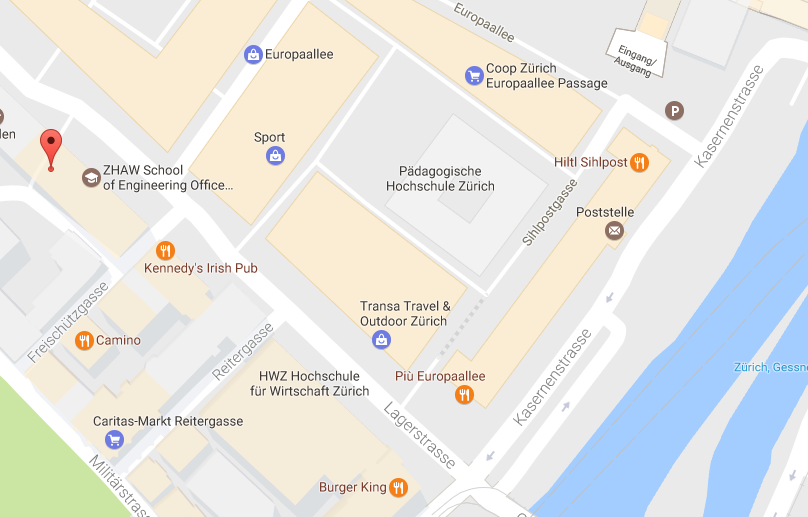
\includegraphics[width=1\textwidth]{images/bing-maps-result}
	\caption{Resultat des Geocodings von Bing Maps.}
	\label{fig:proofofconcept:datenvorbereitung:datenerweiterung:geolocation:1}
\end{figure}

\subsection{Datenvorbereitung mit RapidMiner}
Im \cref{sec:recherche:datenvorbereitung} wurde beschrieben, wie die Daten vorbereitet werden sollen. Dieser Abschnitt zeigt auf wie das Program RapidMiner verwendet wurde um diese Vorgaben zu erfüllen. \cref{fig:recherche:rapidminer:1} zeigt den definierte Prozess auf.

%Zuerst werden die Daten aus dem \gls{csv} File geladen. Anschliessend die Attribute gemäss \cref{fig:recherche:attributeinschraenkung:2} eingeschränkt sowie die Diskretisierung entsprechend \cref{fig:recherche:datenvorbereitung:1} und \ref{fig:recherche:datenvorbereitung:2} durchgeführt.

\begin{figure}[htb]
	\begin{subfigure}[t]{1\textwidth}
		\centering
		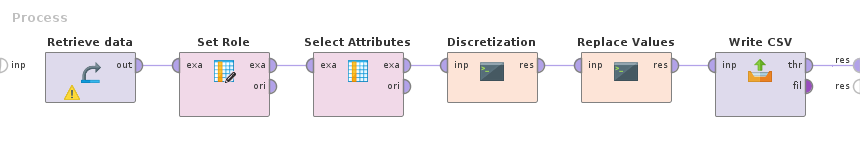
\includegraphics[width=1\textwidth]{images/rapidminer-process}
		\caption{Hauptprocess}
		\label{fig:recherche:rapidminer:1:1}
	\end{subfigure} \\
	\begin{subfigure}[t]{0.5\textwidth}
		\centering
		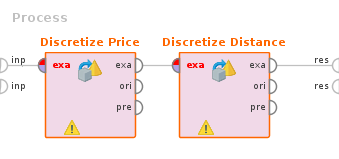
\includegraphics[width=1\textwidth]{images/rapidminer-process-discretization}
		\caption{Subprocess für die Diskretisierung}
		\label{fig:recherche:rapidminer:1:2}
	\end{subfigure}
	\begin{subfigure}[t]{0.8\textwidth}
		\centering
		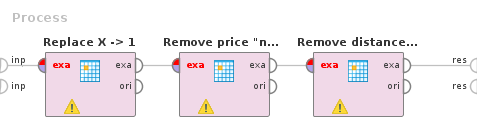
\includegraphics[width=1\textwidth]{images/rapidminer-process-replace-values}
		\caption{Subprocess für die Ersetzung von Attributwerten}
		\label{fig:recherche:rapidminer:1:3}
	\end{subfigure}
	\caption{RapidMiner Prozess für die Vorbereitung der Daten}
	\label{fig:recherche:rapidminer:1}
\end{figure}

 In \ref{fig:recherche:rapidminer:1:1} wird der Hauptprozess gezeigt wie er im RapidMiner definiert wurde. Nachfolgend werden die einzelnen Schritte 
 \begin{itemize}
 	\item Retrieve data: Lädt die Buchungen aus der Datenquelle damit diese bearbeitet werden können. 
 	\item Filter Exapmles: \todo{Filter Example}.
 	\item Select Attribute: Entfernt alle Attribute welche nicht in der \cref{fig:recherche:attributeinschraenkung:2} ausfgewählführt werden, sind die Informationen nachher voll anonymisiert und können auch veröffentlicht werden. Der letzte Schritt schreibt das Resultat in ein \gls{csv} File damit es nachher weiterverwendet werden kann.
 	\item Generate ID: Generiert eine ID für die eindeutige Identifikation der Buchungen.
 	\item Normalize: Normiert nummerische Werte auf einen Interval $0 \leq x \leq 1$ (siehe \cref{sec:recherche:datenvorbereitung:normierung} \nameref{sec:recherche:datenvorbereitung:normierung}).
 	\item Weeklyprice: Berechnet den Wochenpreis einer Buchung (siehe \cref{sec:recherche:datenvorbereitung:normierung} \nameref{sec:recherche:datenvorbereitung:normierung}).
 	\item Discretization: Ist ein Unterprozess welcher in \cref{fig:recherche:rapidminer:1:2} dargestellt ist.
	 	\begin{itemize}
	 		\item Discretize Price: Diskretiert die Preise gemäss \cref{fig:recherche:datenvorbereitung:2}. Die Preisspannen die nicht im Resultat verwendet werden sollen werden später im Schritt "`Replace Values"' entfernt.
	 		\item Discretize Distance: Diskretiert die Distanzen gemäss \cref{fig:recherche:datenvorbereitung:1}. Distanzspannen die nicht im Resultat verwendet werden sollen werden später im Schritt "`Replace Values"' entfernt.
	 	\end{itemize}
 	\item Replace Values: Ist ein Unterprozess welcher in \cref{fig:recherche:rapidminer:1:3} dargestellt ist.
 		\begin{itemize}
			\item Replace X -> 1 und Replace empty -> 0: Wandelt boolsche Werte in 1 und 0 um (siehe \cref{sec:recherche:datenvorbereitung:boolschewerte} \nameref{sec:recherche:datenvorbereitung:boolschewerte}). 
			\item Remove price ...: \todo{}
 		\end{itemize}
 	\item Remove Price: Entfernt den gesamt Preis der Buchung. Dieser muss beim Schritt "`Select Attribute"' hinzugefügt werden damit der Wochenpreis berechnet werden kann. Im Resultat wird das Attribut jedoch nicht mehr benötig.
 	\item Write CSV: Speichert das Resultat im \gls{csv} Format auf die Festplatte ab.
 \end{itemize}

\section{Architektur}
\label{sec:proofofconcept:architektur}
Hier wird die Architektur des Programmes erläutert. Grundlegen wurde die Applikations nach dem \gls{mvc}-\gls{pattern} aufgebaut und um die Entkoppelung der einzelnen Module zu ermöglichen ein Dependency Injection Framework verwendet. Diese und weitere Punkte werden nachfolgend beschrieben.

\subsection{MVC}
\label{sec:proofofconcept:architektur:mvc}
Mit dem \gls{mvc}-\gls{pattern} wird das Programm in die drei Komponenten Datenmodel (Model), Präsentation (View) und Programmsteuerung (Controller) unterteilt. Ein Controller nimmt die Anfrage vom Browser entgegen und kreiert ein Datenmodel mit Hilfe einer Geschäftslogik. Diese Logik gibt ein Datenmodel zurück welches die Programmsteuerung an die Präsentation übergibt welche sie darstellt.

Das Datenmodel fungiert als Vertrag wie die Daten dargestellt werden müssen. Die Präsentation und die Geschäftslogik kann beliebig verändert und ausgetauscht werden, solange das Model sich nicht ändert. Dies fördert die Wa

Die Abhängigkeiten zwischen dem Controller, dem Model und der Geschäftslogik (business logik) wird im \cref{sec:proofofconcept:packagestruktur} visualisiert.

\section{Struktur}
Um eine Übersicht über die Implementation zu geben werden in diesem Abschnitt zuerst die Packages visualisiert und danach die Klassen. Dies sollte helfen nachfolgende Erklärungen zu den Abläufen des Programms besser zu verstehen.

\subsection{Package-Struktur}
\label{sec:proofofconcept:packagestruktur}
Ein Package gruppiert ähnliche Klassen und Interfaces zusammen. Man kann sich ein Package vorstellen wie ein Ordner auf dem Computer. Die Struktur dieser Gruppen sowie deren Verwendung untereinander wird in \cref{fig:proofofconcept:packagestruktur:1} aufgezeigt.
\begin{figure}[H]
	\RawFloats
	\centering
	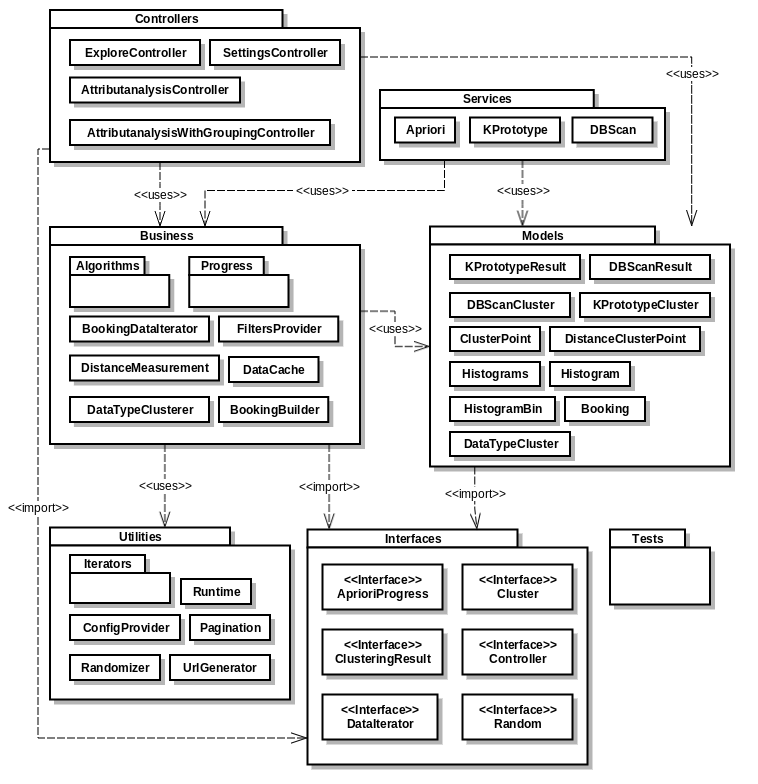
\includegraphics[width=1\textwidth]{images/diagram-package-diagram}
	\caption{Package-Struktur}
	\label{fig:proofofconcept:packagestruktur:1}
\end{figure}

Die Struktur der Packages ist so ausgelegt, dass sie von oben nach unten fliesst. Sprich ein oberes Packet kann ein unteres verwenden, jedoch nicht umgekehrt. Einstiegspunkte für die Ausführung des Programmes sind die Klassen in den Packages Controllers und Services. Ersteres wird vom Benutzer verwendet wenn er eine Seite angezeigt haben möchte. Die Services sind für die Hintergrundprozesse verantwortlich und führen eine Analyse der verschiedenen Algorithmen durch. Nachfolgend werden die einzelnen Packages erklärt.

\begin{itemize}
	\item Controllers: Nehmen die Anfragen eines Benutzers entgegen und verarbeiten diese. Dazu verwenden sie Klassen aus dem Business welches die Models zurückliefert welche schlussendlich dargestellt werden sollen.\todo{cref?}
	\item Services: Führen die verschiedenen Analysen durch. Sie sind so ausgelegt dass sie als eigenständiger Prozess im Hintergrund ausgeführt werden können.\todo{cref}
	\item Business: Beinhaltet die Geschäftlogik, was in dieser Arbeit die Algorithmen umfasst, sowie alles was mit den Models interagiert. Demnach die Algorithmen selber (im Unterpacket "`Algorithms"'), die Distanzmessung (Klasse DistanceMeasurement), den Datenzugriff (Klasse BookingDataIterator), etc.\todo{cref}
	\item Models: Klassen für die Datenhaltung welche möglichst wenig Logik beinhalten.\todo{cref}
	\item Utilities: Beinhalten Logik die nichts mit den Algorithmen zu tun hat und keine Models verwendet. Diese Klassen können für sich selber in einem anderen Projekt wiederverwendet werden.
	\item Interfaces: Alle verwendeten Interfaces.
	\item Tests: UnitTests\todo{cref}
\end{itemize}

\section{Kommunikationsablauf}
\label{sec:proofofconcept:kommunikationsablauf}
In \cref{fig:proofofconcept:kommunikationsablauf:1} wird der Kommunikationsablauf aufgezeigt, welcher zwischen dem Server und dem Browser des Benutzers stattfindet. Sobald der Benutzer eine Analyse startet wird eine Anfrage an den Server gestellt. Dieshalb werden alle Werteer erstellt einen Hintergrundprozess welcher die Analyse durchführt und gibt danach diskretiert und die zu ignorierenden nachher entfernt.
Der Hintergrundprozess führt die Analyse durch und schreibt periodisch einen Zwischenstand im \gls{html}-Format in eine Datei.

In \cref{fig:proofofconcept:kommunikationsablauf:1} wird der Kommunikationsablauf aufgezeigt, welcher zwischen dem Webserver und dem Browser des Benutzers stattfindet. Sobald der Benutzer eine Analyse startet wird eine Anfrage an den Server gestellt. Dieser erstellt einen Hintergrundprozess welcher die Analyse durchführt und gibt danach direkt eine Antwort an den User zurück. 

Der Hintergrundprozess führt die Analyse durch und schreibt periodisch einen Zwischenstand im \gls{html}-Format in eine Datei.

Sobald die Analyse vom Server angestossen wurde kann dieser eine Rückmeldung zum Benutzer senden mit der Nachricht, dass die Analyse gestartet wurde. Der Browser des User beginnt darauf hin, die \gls{html}-Datei auf dem Server nach dem Zwischenstand abzufragen bis die Analyse beendet ist.
\begin{figure}[H]
	\RawFloats
	\centering
	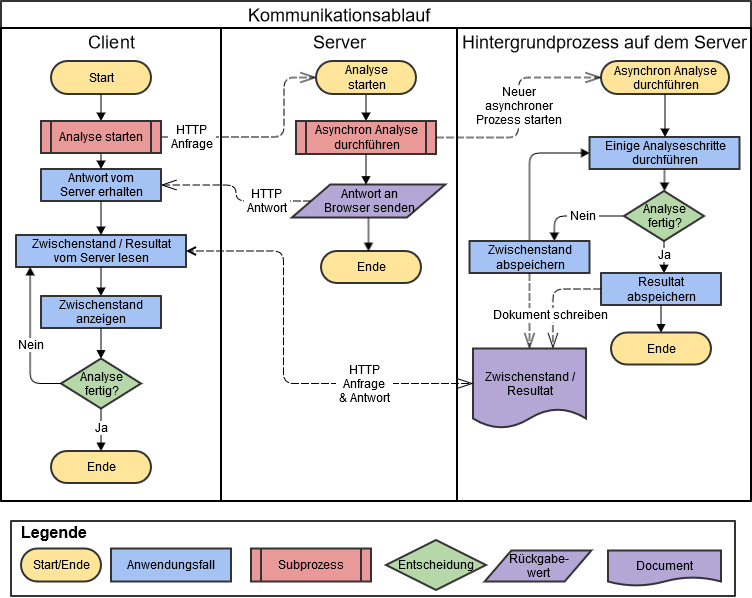
\includegraphics[width=1\textwidth]{images/diagram-communication-flow}
	\caption{Kommunikationsablauf}
	\label{fig:proofofconcept:kommunikationsablauf:1}
\end{figure}

Eine Webanfrage hat normalerweise eine obere Laufzeitgrenze von 30 Sekunden. Bis dann muss der Server eine Antwort liefern, sonst wird dem Benutzer eine Fehlermeldung angezeigt und der Prozess auf dem Server gestoppt. Da die Analyse, je nach Datenmenge, einige Minuten bis Stunden dauern kann musste dafür eine Lösung gefunden werden. Dank des Hintergrundprozesses kann der Server rasch eine Antwort liefern, der Browser dem Benutzer eine Meldung anzeigen und die Analyse länger als 30 Sekunden laufen.

\section{Programmablauf}
Im \cref{sec:proofofconcept:kommunikationsablauf} wurde der Ablauf zwischen dem Benutzer und dem Server illustriert. Hier werden die Abläufe auf dem Webserver sowie der Hintergrundprozesse erläutert.

\subsection{Webserver}
\label{sec:proofofconcept:architektur:webserver}
Der Webserver nimmt einen Request des Users entgegen und verarbeitet diesen. Der Ablauf wird in \cref{fig:proofofconcept:architektur:webserver:1} visualisiert.

\begin{figure}[H]
	\centering
	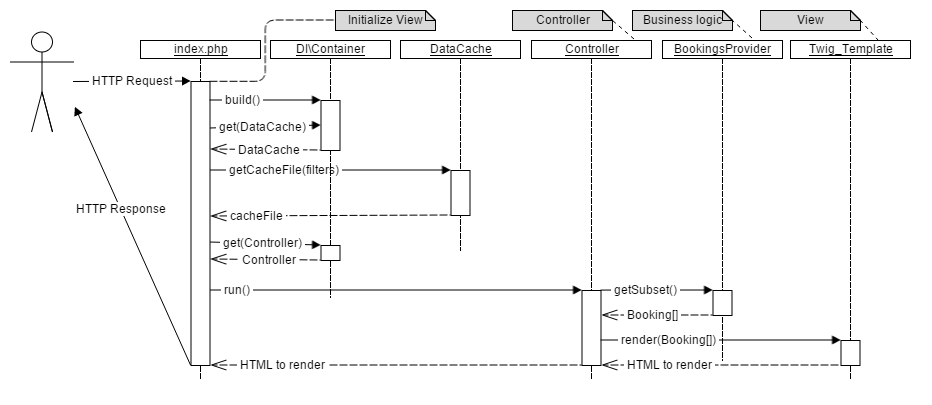
\includegraphics[width=1\textwidth]{images/diagram-sequence-controllers}
	\caption{Sequenzdiagramm für den Ablauf einer "`Explore"'-Anfrage}
	\label{fig:proofofconcept:architektur:webserver:1}
\end{figure}

Aufgerufen wird stets die Datei "`index.php"'. Diese Initialisiert zuerst den dependency injection Container (siehe \cref{sec:proofofconcept:dependency-injection} \nameref{sec:proofofconcept:dependency-injection}) und zwischenspeichert die Datenquelle für die vom Benutzer übergebenen Filterkriterien (siehe \cref{sec:proofofconcept:caching} \nameref{sec:proofofconcept:caching}).

Danach wird der Controller aufgerufen welcher den Request des Benutzers behandelt (siehe \cref{sec:proofofconcept:architektur:mvc} \nameref{sec:proofofconcept:architektur:mvc}). Der Controller führt die Geschäftslogik aus (im obigen Beispiel ist dies die Klasse "`BookingsProvider"') und übergibt das Resultat an die View welche für die Darstellung der Daten zuständig ist. Der Rückgabewert wird dann dem Benutzer im Browser angezeigt.

Dieser Ablauf ist gültig für die "`Explore"'-Ansicht, auf welcher der User die Buchungen einsehen kann. Wenn ein Algorithmus ausgeführt werden soll fällt die Geschäftslogik weg und es wird stattdessen ein Hintergrundprozess gestartet, welcher diese ausführt.

\subsection{Hintergrundprozesse}
\label{sec:proofofconcept:architektur:hintergrundprozesse}
In diesem Abschnitt wird erklärt wie die Hintergrundprozesse angestossen werden sowie deren Abläufe beschrieben. Letzteres wird mit \gls{uml} Sequenzdiagrammen verbildlicht. Die Implementation der Algorithmen selber wird hier nicht genauer beschrieben. Zum einen sind diese im \cref{sec:recherche:algorithmen} bereits dokumentiert und wurden hier entsprechend umgesetzt. Zum anderen würde ein Sequenzdiagramm der Algorithmen zu gross ausfallen und würde deshalb nicht zum Verständnis beitragen können.

Nötig sind die Hintergrundprozesse um die Laufzeit-Limite von Prozessen in einem Webserver zu umgehen. Weitere Informationen hierzu werden im \cref{sec:proofofconcept:kommunikationsablauf} gegeben.

\subsubsection{Anstossen der Hintergrundprozessen}
Die Hintergrundprozesse werden von den Controllern angestossen. Es wird ein Kommandozeilen-Befehl ausgeführt welcher im folgender Ansicht beispielhaft am Apriori-Algorithmus aufgezeigt wird.

\blockquote[]{
php /Services/Apriori/apriori.php ``stars=4,country=Switzerland'' > /Services/Apriori/wip/output.txt 2>\&1 \& echo \$! > /pidfile.txt
}

Zur erklärung dieses Befehles wird er aufgebrochen:
\begin{itemize}
	\item \textbf{php}: Es wird der Befehl "`PHP"' ausgeführt welcher ein PHP Programm startet.
	\item \textbf{/Services/Apriori/apriori.php}: Das auszuführende PHP Programm. Hier die Apriori Analyse.
	\item \textbf{``stars=4,country=Switzerland''}: Parameter die an das "`apriori.php"' Programm übergeben werden. In diesem Beispiel sind das die Filterkriterien des Benutzers.
	\item \textbf{> /Services/Apriori/wip/output.txt}: Mit "`>"' wird die Standartausgabe des Programmes definiert. Jegliche Ausgabe des Programmes wird hiermit in die Datei "`output.txt"' geschrieben.
	\item \textbf{2>\&1}: Mit "`2>"' wird gesagt wohin Fehlemeldungen geschrieben werden. \&1 gibt an dass es an den selben Ort wie die Standartausgabe gespeichert werden soll. Also auch ins "`output.txt"'.
	\item \textbf{\&}: Durch das \& wird der Befehl im Hintergrund ausgeführt. Wenn dies nicht angegeben wird würde das Programm, welches den "`PHP"' Befehl gestartet hat warten, bis das "`apriori.php"' Programm fertig gearbeitet hat.
	\item \textbf{echo \$! > /pidfile.txt}: "echo \$!" gibt die Prozessid des "`apriori.php"' Programmes aus. Mit "`> /pidfile.txt"' wird die Ausgabe (also die Prozessid) in die Datei "`pidfile.txt"' geschrieben.
\end{itemize}

\subsubsection{Ablauf des Apriori-Programmes}
Der Ablauf der Apriori-Analyse wird in \cref{fig:proofofconcept:architektur:hintergrundprozesser:1} verbildlicht.

\begin{figure}[H]
	\centering
	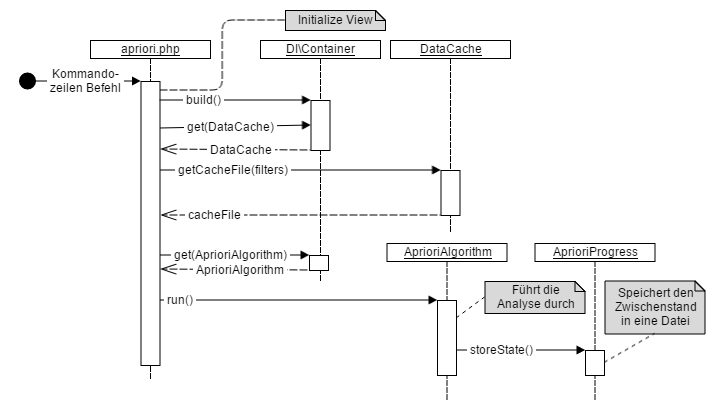
\includegraphics[width=1\textwidth]{images/diagram-sequence-apriori}
	\caption{Sequenzdiagramm für die Initialisierung der Apriori-Analyse}
	\label{fig:proofofconcept:architektur:hintergrundprozesser:1}
\end{figure}

Der Anfang mit dem Erstellen des "`Container"' und dem Caching ist gleich wie in \cref{fig:proofofconcept:architektur:webserver:1}. Das "`apriori.php"' Programm ruft danach den Apriori-Algorithmus auf welcher sein Resultat periodisch in eine Datei schreibt (siehe \cref{sec:proofofconcept:kommunikationsablauf} \nameref{sec:proofofconcept:kommunikationsablauf}). Dies ermöglicht dem Algorithmus regelmässig einen Zwischenstand abzuspeichern welcher dem Benutzer angezeigt werden kann.

\subsubsection{Ablauf der Clustering-Programmen}
Der Ablauf der Clustering-Analysen ist identisch zu jenem des Apriori-Algorithmus, mit zwei Ausnahmen. Zum einen wird vor dem "`AprioriAlgorithm"' der "`KPrototypeAlgorithm"' ausgeführt wird, welcher ein "`KPrototypeResult"' zurück liefert. 
Zum anderen wird dem "`AprioriAlgorithm"' das Resultat vom KPrototype als Parameter übergeben. Dadurch ist em dem "`KPrototypeAlgorithm"' möglich, nur die Elemente eines Clusters zu analysieren und nicht die gesamte Datenmenge. 
Es wurde bewusst entschieden, dass der "`AprioriAlgorithm"' aus der kprototype.php Datei hinaus aufgerufen wird. Dadurch kann zukünftig dieser Algorithmus einfach durch eine Alternative ausgetauscht werden.
Abgebildet ist der Ablauf in \cref{fig:proofofconcept:architektur:hintergrundprozesser:2}. 
\begin{figure}[H]
	\centering
	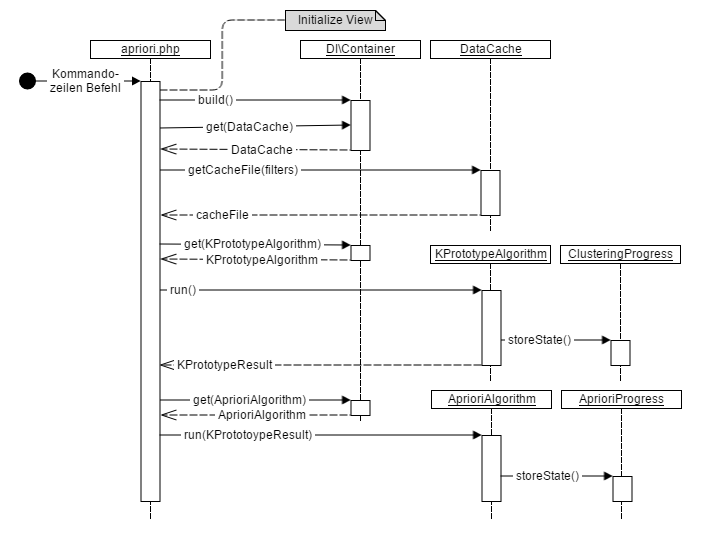
\includegraphics[width=1\textwidth]{images/diagram-sequence-kprototype}
	\caption{Sequenzdiagramm für die Initialisierung der KPrototype-Analyse}
	\label{fig:proofofconcept:architektur:hintergrundprozesser:2}
\end{figure}

Auf ein Sequenzdiagramm für den DBSCAN-Algorithmus wird hier verzichtet, denn die Visualisierung des DBSCAN-Ablaufs ist identisch wie jener vom KPrototype. Lediglich die Namen der aufgerufenen Klassen müssten angepasst werden.

\section{Dependency Injection mit PHP-DI}
\label{sec:proofofconcept:dependency-injection}
Bei der Dependency Injection handelt es sich um ein \gls{pattern}
das zum Ziel hat, eine möglichst niedrige Kopplung zu erreichen. Dies bedeutet, dass eine Klasse so wenig Abhängigkeiten wie möglich zu anderen Komponenten aufweisen soll. Dadurch können einzelne Klassen einfacher ausgetauscht werden washt die Wartbarkeit des Systems erhöht sowie die Leserlichkeit des Codes fordert. Dies soll anhand eines Beispieles aufgezeigt werden.

\begin{lstlisting}[language=php]
var _x = $\textdollar$y
\end{lstlisting}

\begin{lstlisting}[language=php]
class Car {
	public $\textdollar$engine;
	
	public function __construct() {
		$\textdollar$this->engine = new V6Engine();
	}
	
	public function accelerate() {
		$\textdollar$this->engine->accelerate();
	}
}
\end{lstlisting}

Im obigen Code wird eine Klasse Car erstellt in dessen Konstruktor ein V6 Motor instanziiert  wird. Der Code ist jetzt direkt gekoppelt mit der Klasse V6Engine. Wenn ein Auto mit einem V4Engine erstellt werden soll muss die Klasse entsprechend angepasst werden. 


\begin{lstlisting}[language=php]
class Car {
	public $\textdollar$engine;
	
	public function __construct(Engine engine) {
		$\textdollar$this->engine = engine;
	}
	
	public function accelerate() {
		$\textdollar$this->engine->accelerate();
	}
}
\end{lstlisting}

Hier wurde die Klasse so angepasst, dass der Konstruktor keinen Motor erstellt, sondern diesen über die Parameter übernimmt. So kann von aussen gesteuert werden, welchen Engine das Auto beinhaltet. 

In der Arbeit werden alle Komponenten über Dependency Injection in Klassen hineingereicht. Die einzige Ausnahme sind die Models, weshalb sie auch möglichst wenig Logik beinhalten sollten (siehe \cref{sec:proofofconcept:packagestruktur} \nameref{sec:proofofconcept:packagestruktur}). Dies kann besonders gut mit den Iteratoren veranschaulicht werden. Die Klasse "`BookingDataIterator"' nimmt ein Interface "`DataIterator"' entgegen. Es gibt 5 Klassen welche dieses Interface implementieren wovon 3 hier erläutert werden:
\begin{itemize}
	\item LoadAllCsvDataIterator: Lädt alle Buchungsdaten aus einem File ins Memory und iteriert dann über die einzelnen Instanzen.
	\item LoadIncrementalCsvDataIterator: Lädt eine Instanz nach der anderen aus dem File.
	\item LoadRedisDataIterator: Lädt eine Instanz nach der anderen aus einer Redis Datenbank (In Memory Datenban)\todo{cref}
\end{itemize}

Es gibt demnach 3 verschiedene Möglichkeiten, wie auf die Daten zugegriffen werden kann. Mittels Dependency Injection kann nun von aussen bestimmt werden, wie der "`BookingDataIterator"' auf die Daten zugreift.

Für das Dependency Injection \gls{pattern}
 wird das Framework PHP-DI verwendet (siehe \url{http://php-di.org/}). In der ersten geladenen Datei wird der gesamte Objektgraph aufgebaut. Dort wird bestimmt, welche Klasse in den "`BookingDataIterator"' übergeben wird. Ein Beispiel wird nachfolgend präsentiert:
 
\begin{lstlisting}[language=php]
$\textdollar$builder = new DI\ContainerBuilder();
$\textdollar$builder->addDefinitions([
    [...]
    DataIterator::class => DI\object(LoadIncrementalCsvDataIterator::class),
    [...]
]);
$\textdollar$container = $\textdollar$builder->build();
$\textdollar$apriori = $\textdollar$container->get('AprioriAlgorithm');
$\textdollar$apriori->run();
\end{lstlisting}

Zuerst wird ein "`ContainerBuilder"' erstellt. Auf diesem wird definiert, dass für das "`DataIterator"' Interface die Klasse "`LoadIncrementalCsvDataIterator"' verwendet werden soll. Danach wird auf Zeile 7 ein "`Container"' erstellt und anschliessend eine Instanz der Klasse "`AprioriAlgorithm"' angefordert. Der Container analysiert die Klasse und sieht dass ein "`DataIterator"' erwartet wird und reicht deshalb ein "`LoadIncrementalCsvDataIterator"' in den "`AprioriAlgorithm"' rein. Somit kann auf oberster Ebene gesteuert werden, welche Klassen wo übergeben werden.

Als erfreulicher Nebeneffekt erleichtert dies die Entwicklung von UnitTests massiv (\todo{cref}).

\section{Caching}
\label{sec:proofofconcept:caching}